\hypertarget{Classes_8h}{
\section{Classes.h File Reference}
\label{Classes_8h}\index{Classes.h@{Classes.h}}
}


This graph shows which files directly or indirectly include this file:\nopagebreak
\begin{figure}[H]
\begin{center}
\leavevmode
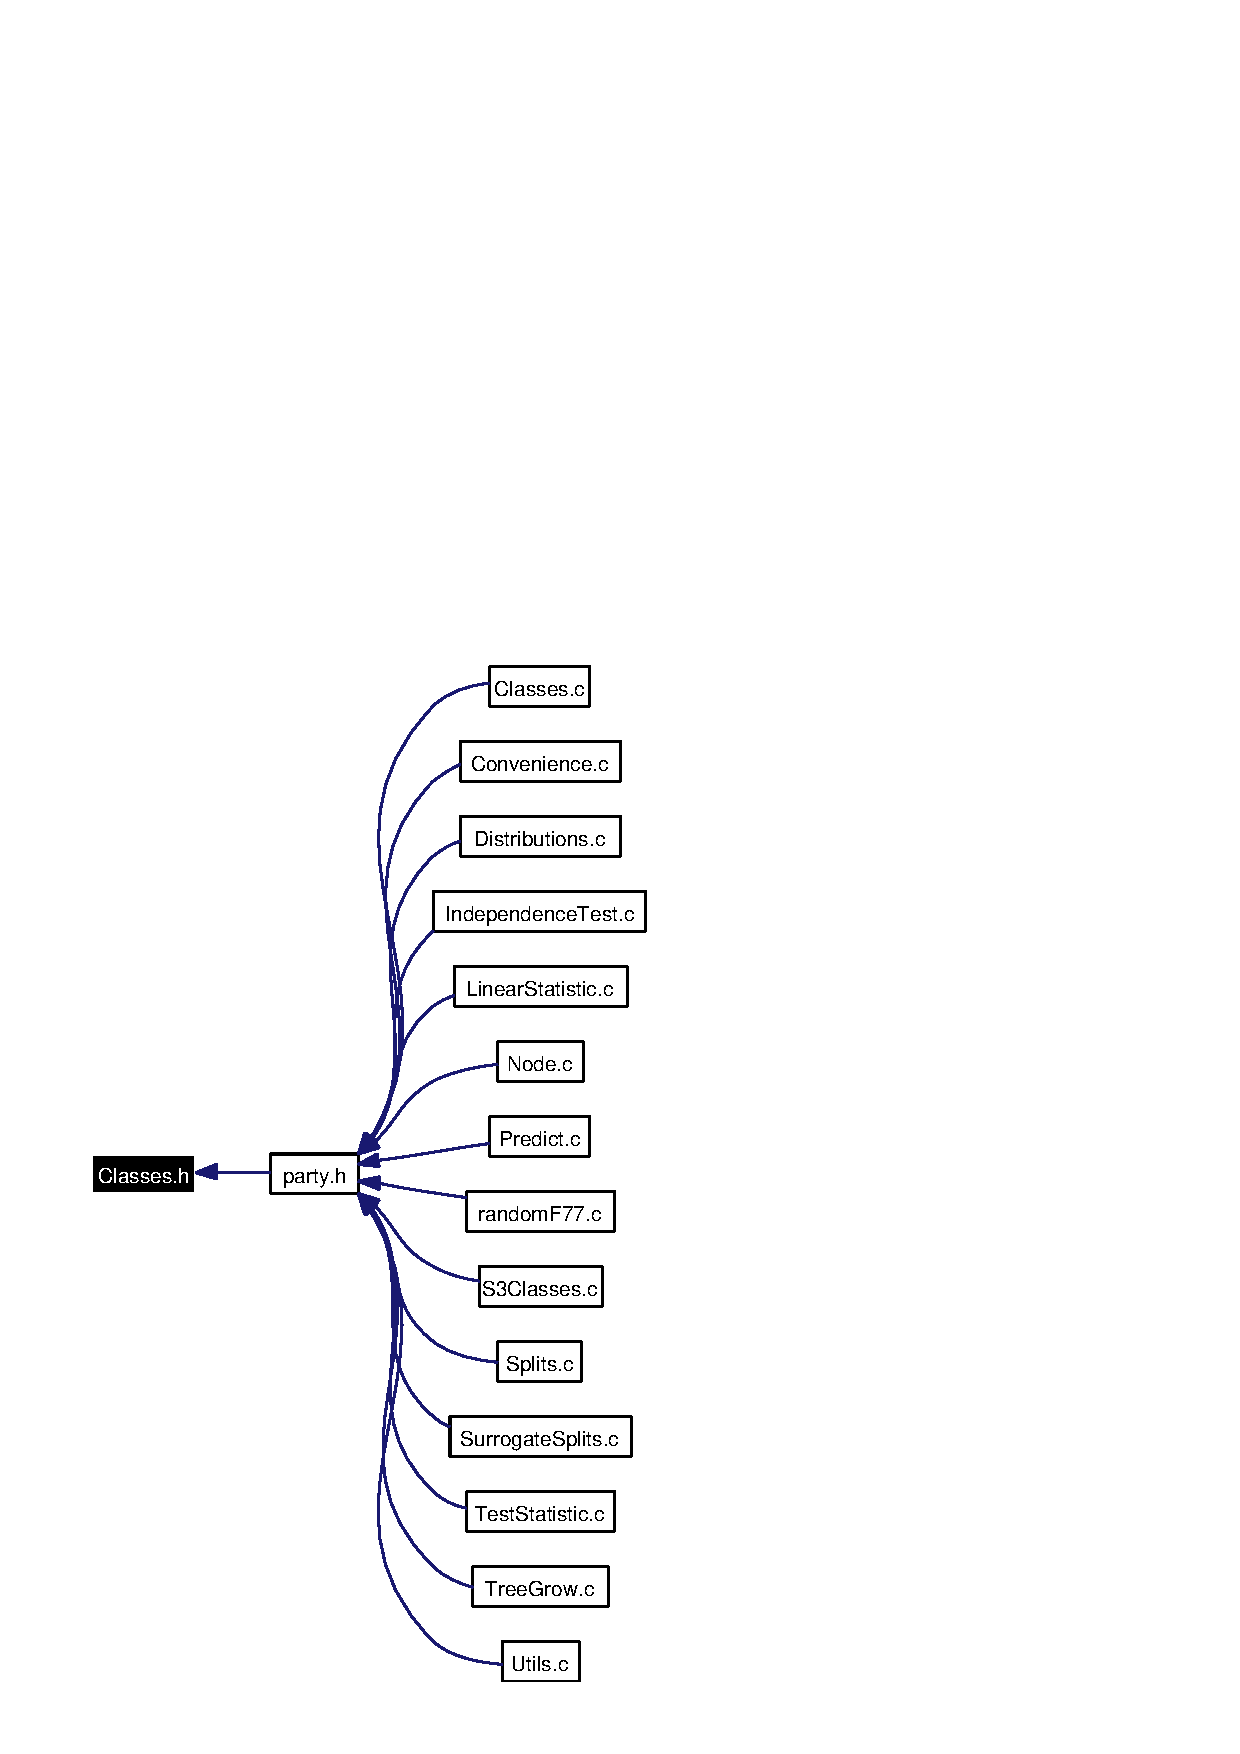
\includegraphics[width=420pt]{Classes_8h__dep__incl}
\end{center}
\end{figure}
\subsection*{Functions}
\begin{CompactItemize}
\item 
int \hyperlink{Classes_8h_8bc9164a2291bb7f61c12b79f6bc7c5f}{get\_\-dimension} (SEXP object)
\item 
int \hyperlink{Classes_8h_847e08eb9fce554539de3106ea03e9e2}{get\_\-teststat} (SEXP object)
\item 
double \hyperlink{Classes_8h_aa5df349ffd6e5faccab211ac972722b}{get\_\-tol} (SEXP object)
\item 
int \hyperlink{Classes_8h_309a9064403a71aba540cad646ba5854}{get\_\-pvalue} (SEXP object)
\item 
int \hyperlink{Classes_8h_b0fc0f7fb33f87cfa58cb8c617d946a1}{get\_\-maxpts} (SEXP object)
\item 
double \hyperlink{Classes_8h_4e2233c1c47758c555f99235f60984f0}{get\_\-abseps} (SEXP object)
\item 
double \hyperlink{Classes_8h_a17053ff24db1859af60e2d71baf924c}{get\_\-releps} (SEXP object)
\item 
double \hyperlink{Classes_8h_024b7f74a61afa9b3eb465a98f35584c}{get\_\-minsplit} (SEXP object)
\item 
double \hyperlink{Classes_8h_f7aaeccefe1bfbb1737ac3403a85c8e9}{get\_\-minprob} (SEXP object)
\item 
double \hyperlink{Classes_8h_0794d3cb26a60105140165d6dea3d70d}{get\_\-minbucket} (SEXP object)
\item 
SEXP \hyperlink{Classes_8h_20a55355301b5f90ec48b9114d1ff597}{get\_\-transformation} (SEXP object, int variable)
\item 
SEXP \hyperlink{Classes_8h_9ec50a13a7c7e82143cced16ff4f3968}{get\_\-test\_\-trafo} (SEXP object)
\item 
SEXP \hyperlink{Classes_8h_b86d70ff194260cc9bd391d3ff55b157}{get\_\-predict\_\-trafo} (SEXP object)
\item 
SEXP \hyperlink{Classes_8h_0f91efa916e815ec7d90c6f9516f18e4}{get\_\-variable} (SEXP object, int variable)
\item 
int \hyperlink{Classes_8h_f836613ade2cdc01c401b574fc1e7fdb}{is\_\-nominal} (SEXP object, int variable)
\item 
int \hyperlink{Classes_8h_53608524b90af1655d49496ec5ccbd47}{is\_\-ordinal} (SEXP object, int variable)
\item 
int \hyperlink{Classes_8h_2ea962f10f7adde8ad25429e15cad9d3}{is\_\-censored} (SEXP object, int variable)
\item 
int \hyperlink{Classes_8h_50548fbe6024d9a7118db3fce5085fd9}{has\_\-missings} (SEXP object, int variable)
\item 
SEXP \hyperlink{Classes_8h_fd6cfc2dd239b138d91e92a8ce9353f8}{get\_\-missings} (SEXP object, int variable)
\item 
SEXP \hyperlink{Classes_8h_a160107e2d687d3fa2411af7e25763ef}{get\_\-ordering} (SEXP object, int variable)
\item 
SEXP \hyperlink{Classes_8h_0e317821da8f3bc0fb6da5006abb81f6}{get\_\-levels} (SEXP object, int variable)
\item 
SEXP \hyperlink{Classes_8h_ba4726f56726372030e1e104b2f2b076}{get\_\-scores} (SEXP object, int variable)
\item 
SEXP \hyperlink{Classes_8h_e3c823841d28ac07932df6cf545563c5}{get\_\-whichNA} (SEXP object, int variable)
\item 
SEXP \hyperlink{Classes_8h_31bf6c4f0764bc42b413cc319a0f9ec2}{get\_\-varmemory} (SEXP object, int variable)
\item 
int \hyperlink{Classes_8h_45df17685bc6c95d03fb65b6f6214de0}{get\_\-nobs} (SEXP object)
\item 
int \hyperlink{Classes_8h_9117d8f57ea1378c725c7299d6cc2923}{get\_\-ninputs} (SEXP object)
\item 
SEXP \hyperlink{Classes_8h_266fda49284a556bbe8aaa80e348a3ca}{get\_\-weights} (SEXP object)
\item 
int \hyperlink{Classes_8h_7f1c5e96481b726312de51ca7c6ef924}{get\_\-testtype} (SEXP object)
\item 
int \hyperlink{Classes_8h_af696af616c142e55ea0758690d20d7c}{get\_\-nresample} (SEXP object)
\item 
SEXP \hyperlink{Classes_8h_a7f64a77df0cfbcae9428aa6684a1ad1}{get\_\-varctrl} (SEXP object)
\item 
SEXP \hyperlink{Classes_8h_d914bd038dca4d2a1b9847f46bdb78f9}{get\_\-splitctrl} (SEXP object)
\item 
SEXP \hyperlink{Classes_8h_43fe1d056590d0d70d3a72beda13963e}{get\_\-gtctrl} (SEXP object)
\item 
double \hyperlink{Classes_8h_3578ef4fb8f0c3ecd7d166687acde94a}{get\_\-mincriterion} (SEXP object)
\item 
int \hyperlink{Classes_8h_79a38a57d0a4fbf5d7df55bf9a1dc66d}{get\_\-randomsplits} (SEXP object)
\item 
SEXP \hyperlink{Classes_8h_7d89658acc342f53100657fb4984fe80}{get\_\-mtry} (SEXP object)
\item 
SEXP \hyperlink{Classes_8h_3598986a5115e969e9d435c5036dcecf}{get\_\-dontuse} (SEXP object)
\item 
SEXP \hyperlink{Classes_8h_3c02aa6a5a00bc0ca460e78540fa064c}{get\_\-dontusetmp} (SEXP object)
\item 
int \hyperlink{Classes_8h_c7779f00dc36c589dd24e3b4f6247be3}{get\_\-stump} (SEXP object)
\item 
int \hyperlink{Classes_8h_b89e4da7a60580c3adbe7c4f4935581c}{get\_\-maxsurrogate} (SEXP object)
\item 
SEXP \hyperlink{Classes_8h_a88e9e2563188b5500b48a6efaee9734}{get\_\-tgctrl} (SEXP object)
\item 
SEXP \hyperlink{Classes_8h_3a0ec14f5047b8c9bf8d8e6ba3c6e306}{get\_\-splitstatistics} (SEXP object)
\item 
int \hyperlink{Classes_8h_2c17918334d53626178a38518f9f25ff}{get\_\-savesplitstats} (SEXP object)
\item 
int \hyperlink{Classes_8h_871d0c7dc9639a559b15a8790268063d}{check\_\-depth} (SEXP object, int depth)
\item 
int \hyperlink{Classes_8h_899349b79a444c39ff23856bd802e096}{get\_\-ntree} (SEXP object)
\item 
int \hyperlink{Classes_8h_2c31f2150a75ae67496074deeaea1f96}{get\_\-replace} (SEXP object)
\item 
double \hyperlink{Classes_8h_3367507eb875c7601cdb9d77f15b5871}{get\_\-fraction} (SEXP object)
\end{CompactItemize}
\subsection*{Variables}
\begin{CompactItemize}
\item 
SEXP \hyperlink{Classes_8h_f0a2dc8073174e68e71d4d19266bab22}{PL2\_\-expectationSym}
\item 
SEXP \hyperlink{Classes_8h_e033132aed4900e99ec36faf7352ea34}{PL2\_\-covarianceSym}
\item 
SEXP \hyperlink{Classes_8h_e36e22e2f694307e4d5af6dade35abc6}{PL2\_\-linearstatisticSym}
\item 
SEXP \hyperlink{Classes_8h_4d117ff485f06bee9902f99246ac9c04}{PL2\_\-expcovinfSym}
\item 
SEXP \hyperlink{Classes_8h_1f0d5394a08065f5e1a54608dac5916d}{PL2\_\-expcovinfssSym}
\item 
SEXP \hyperlink{Classes_8h_72d079f51635b70b0a19dfe3bc6716c8}{PL2\_\-sumweightsSym}
\item 
SEXP \hyperlink{Classes_8h_b993e9eabf03921afdda536cd0d03ef3}{PL2\_\-dimensionSym}
\item 
SEXP \hyperlink{Classes_8h_6281f5e20196f03b8ca82137e9f0bee7}{PL2\_\-MPinvSym}
\item 
SEXP \hyperlink{Classes_8h_2369f12a0df12fcae97775c41b461b63}{PL2\_\-rankSym}
\item 
SEXP \hyperlink{Classes_8h_191eafdb9f05be24507087e4a0cb656d}{PL2\_\-svdmemSym}
\item 
SEXP \hyperlink{Classes_8h_f132d3e468f57f7d311f7d682e28d59d}{PL2\_\-methodSym}
\item 
SEXP \hyperlink{Classes_8h_e5f84a192b44654299d3b2c6f7febb0b}{PL2\_\-jobuSym}
\item 
SEXP \hyperlink{Classes_8h_faaa2e8cc7b0f2244d84dcd517ba3bf6}{PL2\_\-jobvSym}
\item 
SEXP \hyperlink{Classes_8h_d81981007d31ea647673010bdd41bcc2}{PL2\_\-uSym}
\item 
SEXP \hyperlink{Classes_8h_7362d58f9bd0581cf6c7b584d2783167}{PL2\_\-vSym}
\item 
SEXP \hyperlink{Classes_8h_d9bc9a01dae6a98d2709e4d8b26124e8}{PL2\_\-sSym}
\item 
SEXP \hyperlink{Classes_8h_d088d7d8474d9c927044da9ba5f37837}{PL2\_\-pSym}
\item 
SEXP \hyperlink{Classes_8h_e430cc10639e774cf1b3daa8bbbe5496}{PL2\_\-teststatSym}
\item 
SEXP \hyperlink{Classes_8h_969daa58978bef428c6c6938e5113509}{PL2\_\-pvalueSym}
\item 
SEXP \hyperlink{Classes_8h_824c4bd02d12a3dd1d316a51fe622b0c}{PL2\_\-tolSym}
\item 
SEXP \hyperlink{Classes_8h_87248987fad9ad3b05be6d24eba22886}{PL2\_\-maxptsSym}
\item 
SEXP \hyperlink{Classes_8h_c4c2f757e83d183b6a85addfb8713c4c}{PL2\_\-absepsSym}
\item 
SEXP \hyperlink{Classes_8h_1b283af10ddc0589b96baa42d609f237}{PL2\_\-relepsSym}
\item 
SEXP \hyperlink{Classes_8h_109785d63340f9ae8e21f0b6dde2aa20}{PL2\_\-minsplitSym}
\item 
SEXP \hyperlink{Classes_8h_c973393fe44233f4b23dc2f11a30f908}{PL2\_\-minbucketSym}
\item 
SEXP \hyperlink{Classes_8h_956e5ea52c0c35b429e14619e7f94ee5}{PL2\_\-minprobSym}
\item 
SEXP \hyperlink{Classes_8h_94e141e6d1a1315e28d142860b5f987e}{PL2\_\-variablesSym}
\item 
SEXP \hyperlink{Classes_8h_6f387307dcb17869091e08e6c7d5a5c5}{PL2\_\-transformationsSym}
\item 
SEXP \hyperlink{Classes_8h_7fc0ba403124f5d582b0e5abd13f4fb4}{PL2\_\-is\_\-nominalSym}
\item 
SEXP \hyperlink{Classes_8h_619562059f34e6d80cac945f03efd16c}{PL2\_\-is\_\-ordinalSym}
\item 
SEXP \hyperlink{Classes_8h_b599a0472b4568fbc3111f315ebb035f}{PL2\_\-is\_\-censoredSym}
\item 
SEXP \hyperlink{Classes_8h_6a6f78bf6df3ce35b0d6315db7e60165}{PL2\_\-orderingSym}
\item 
SEXP \hyperlink{Classes_8h_780ff4fae7d4b234b757caf5cec27a35}{PL2\_\-levelsSym}
\item 
SEXP \hyperlink{Classes_8h_68c23c34260e4a4863e5c0caf2b3b411}{PL2\_\-scoresSym}
\item 
SEXP \hyperlink{Classes_8h_6cad742d32f0ac66eb12db5312c062b6}{PL2\_\-has\_\-missingsSym}
\item 
SEXP \hyperlink{Classes_8h_48fecaa469261c6beb2abb11970a29ef}{PL2\_\-whichNASym}
\item 
SEXP \hyperlink{Classes_8h_16a47750f3b0a7e3261132bc24c1cdde}{PL2\_\-test\_\-trafoSym}
\item 
SEXP \hyperlink{Classes_8h_727b86d73186990d5620eb01e39b2707}{PL2\_\-predict\_\-trafoSym}
\item 
SEXP \hyperlink{Classes_8h_eb411e47896a840cc77dd3cae74533d8}{PL2\_\-nobsSym}
\item 
SEXP \hyperlink{Classes_8h_4cc863cbaafba964bbc10a4ad7b90c72}{PL2\_\-ninputsSym}
\item 
SEXP \hyperlink{Classes_8h_adb3a293553f93d6233d9ba4ab7d1039}{PL2\_\-linexpcov2sampleSym}
\item 
SEXP \hyperlink{Classes_8h_81fa0afba4ad786166ef0872c842a9db}{PL2\_\-weightsSym}
\item 
SEXP \hyperlink{Classes_8h_6b4204d372191db8c7fb0210bfce8f6a}{PL2\_\-varmemorySym}
\item 
SEXP \hyperlink{Classes_8h_9ad5f5cd65458d95a8ffae2d450ec850}{PL2\_\-responsesSym}
\item 
SEXP \hyperlink{Classes_8h_a0f1db0215808916904d250b11f71edd}{PL2\_\-inputsSym}
\item 
SEXP \hyperlink{Classes_8h_81b84b3f654314ad4bd6885dad350ad3}{PL2\_\-testtypeSym}
\item 
SEXP \hyperlink{Classes_8h_0ca6293b541d65ee9205ef090e3a89c0}{PL2\_\-nresampleSym}
\item 
SEXP \hyperlink{Classes_8h_590494b5bcca46b1624c9cfb40e3fa7a}{PL2\_\-varctrlSym}
\item 
SEXP \hyperlink{Classes_8h_a416b1a8d0e742414f07cecc14b2ff22}{PL2\_\-splitctrlSym}
\item 
SEXP \hyperlink{Classes_8h_3624cf464666d668ac01bd82e1dbb67e}{PL2\_\-gtctrlSym}
\item 
SEXP \hyperlink{Classes_8h_4978acb0c711be68d72823f0e4b6141e}{PL2\_\-mincriterionSym}
\item 
SEXP \hyperlink{Classes_8h_773e1edf30b724c5335c1276ed3c6a6c}{PL2\_\-randomsplitsSym}
\item 
SEXP \hyperlink{Classes_8h_59e6ce8e5bed48dcf9299d9a7bff933d}{PL2\_\-mtrySym}
\item 
SEXP \hyperlink{Classes_8h_38ddf1da2b9d162d074d1f5c6d5c0418}{PL2\_\-dontuseSym}
\item 
SEXP \hyperlink{Classes_8h_60440f0803a2789589834032edcc31f5}{PL2\_\-dontusetmpSym}
\item 
SEXP \hyperlink{Classes_8h_ba1a6d09a1f030c9dea1b11dc46e2f1a}{PL2\_\-stumpSym}
\item 
SEXP \hyperlink{Classes_8h_9b2381d5cefcc57f5fa2e140167ecb9d}{PL2\_\-tgctrlSym}
\item 
SEXP \hyperlink{Classes_8h_8c22189efef525e27fd3793ca37aa109}{PL2\_\-ntreeSym}
\item 
SEXP \hyperlink{Classes_8h_4b88d1bbcab84cb3e7d1e634d9df1af2}{PL2\_\-replaceSym}
\item 
SEXP \hyperlink{Classes_8h_3beca0734adb10de599aa3c2e2d9f329}{PL2\_\-fractionSym}
\end{CompactItemize}


\subsection{Function Documentation}
\hypertarget{Classes_8h_871d0c7dc9639a559b15a8790268063d}{
\index{Classes.h@{Classes.h}!check\_\-depth@{check\_\-depth}}
\index{check\_\-depth@{check\_\-depth}!Classes.h@{Classes.h}}
\subsubsection[{check\_\-depth}]{\setlength{\rightskip}{0pt plus 5cm}int check\_\-depth (SEXP {\em object}, \/  int {\em depth})}}
\label{Classes_8h_871d0c7dc9639a559b15a8790268063d}




Definition at line 346 of file Classes.c.

References PL2\_\-maxdepthSym.

Referenced by C\_\-TreeGrow().\hypertarget{Classes_8h_4e2233c1c47758c555f99235f60984f0}{
\index{Classes.h@{Classes.h}!get\_\-abseps@{get\_\-abseps}}
\index{get\_\-abseps@{get\_\-abseps}!Classes.h@{Classes.h}}
\subsubsection[{get\_\-abseps}]{\setlength{\rightskip}{0pt plus 5cm}double get\_\-abseps (SEXP {\em object})}}
\label{Classes_8h_4e2233c1c47758c555f99235f60984f0}




Definition at line 167 of file Classes.c.

References PL2\_\-absepsSym.

Referenced by C\_\-TeststatPvalue().\hypertarget{Classes_8h_8bc9164a2291bb7f61c12b79f6bc7c5f}{
\index{Classes.h@{Classes.h}!get\_\-dimension@{get\_\-dimension}}
\index{get\_\-dimension@{get\_\-dimension}!Classes.h@{Classes.h}}
\subsubsection[{get\_\-dimension}]{\setlength{\rightskip}{0pt plus 5cm}int get\_\-dimension (SEXP {\em object})}}
\label{Classes_8h_8bc9164a2291bb7f61c12b79f6bc7c5f}




Definition at line 147 of file Classes.c.

References PL2\_\-dimensionSym.

Referenced by C\_\-ConditionalPvalue(), C\_\-Node(), C\_\-TestStatistic(), and R\_\-splitcategorical().\hypertarget{Classes_8h_3598986a5115e969e9d435c5036dcecf}{
\index{Classes.h@{Classes.h}!get\_\-dontuse@{get\_\-dontuse}}
\index{get\_\-dontuse@{get\_\-dontuse}!Classes.h@{Classes.h}}
\subsubsection[{get\_\-dontuse}]{\setlength{\rightskip}{0pt plus 5cm}SEXP get\_\-dontuse (SEXP {\em object})}}
\label{Classes_8h_3598986a5115e969e9d435c5036dcecf}




Definition at line 334 of file Classes.c.

References PL2\_\-dontuseSym.

Referenced by C\_\-GlobalTest().\hypertarget{Classes_8h_3c02aa6a5a00bc0ca460e78540fa064c}{
\index{Classes.h@{Classes.h}!get\_\-dontusetmp@{get\_\-dontusetmp}}
\index{get\_\-dontusetmp@{get\_\-dontusetmp}!Classes.h@{Classes.h}}
\subsubsection[{get\_\-dontusetmp}]{\setlength{\rightskip}{0pt plus 5cm}SEXP get\_\-dontusetmp (SEXP {\em object})}}
\label{Classes_8h_3c02aa6a5a00bc0ca460e78540fa064c}




Definition at line 338 of file Classes.c.

References PL2\_\-dontusetmpSym.

Referenced by C\_\-GlobalTest().\hypertarget{Classes_8h_3367507eb875c7601cdb9d77f15b5871}{
\index{Classes.h@{Classes.h}!get\_\-fraction@{get\_\-fraction}}
\index{get\_\-fraction@{get\_\-fraction}!Classes.h@{Classes.h}}
\subsubsection[{get\_\-fraction}]{\setlength{\rightskip}{0pt plus 5cm}double get\_\-fraction (SEXP {\em object})}}
\label{Classes_8h_3367507eb875c7601cdb9d77f15b5871}




Definition at line 362 of file Classes.c.

References PL2\_\-fractionSym.

Referenced by R\_\-Ensemble().\hypertarget{Classes_8h_43fe1d056590d0d70d3a72beda13963e}{
\index{Classes.h@{Classes.h}!get\_\-gtctrl@{get\_\-gtctrl}}
\index{get\_\-gtctrl@{get\_\-gtctrl}!Classes.h@{Classes.h}}
\subsubsection[{get\_\-gtctrl}]{\setlength{\rightskip}{0pt plus 5cm}SEXP get\_\-gtctrl (SEXP {\em object})}}
\label{Classes_8h_43fe1d056590d0d70d3a72beda13963e}




Definition at line 310 of file Classes.c.

References PL2\_\-gtctrlSym.

Referenced by C\_\-Node().\hypertarget{Classes_8h_0e317821da8f3bc0fb6da5006abb81f6}{
\index{Classes.h@{Classes.h}!get\_\-levels@{get\_\-levels}}
\index{get\_\-levels@{get\_\-levels}!Classes.h@{Classes.h}}
\subsubsection[{get\_\-levels}]{\setlength{\rightskip}{0pt plus 5cm}SEXP get\_\-levels (SEXP {\em object}, \/  int {\em variable})}}
\label{Classes_8h_0e317821da8f3bc0fb6da5006abb81f6}




Definition at line 235 of file Classes.c.

References is\_\-nominal(), is\_\-ordinal(), and PL2\_\-levelsSym.

Referenced by C\_\-Node().

Here is the call graph for this function:\nopagebreak
\begin{figure}[H]
\begin{center}
\leavevmode
\includegraphics[width=102pt]{Classes_8h_0e317821da8f3bc0fb6da5006abb81f6_cgraph}
\end{center}
\end{figure}
\hypertarget{Classes_8h_b0fc0f7fb33f87cfa58cb8c617d946a1}{
\index{Classes.h@{Classes.h}!get\_\-maxpts@{get\_\-maxpts}}
\index{get\_\-maxpts@{get\_\-maxpts}!Classes.h@{Classes.h}}
\subsubsection[{get\_\-maxpts}]{\setlength{\rightskip}{0pt plus 5cm}int get\_\-maxpts (SEXP {\em object})}}
\label{Classes_8h_b0fc0f7fb33f87cfa58cb8c617d946a1}




Definition at line 163 of file Classes.c.

References PL2\_\-maxptsSym.

Referenced by C\_\-TeststatPvalue().\hypertarget{Classes_8h_b89e4da7a60580c3adbe7c4f4935581c}{
\index{Classes.h@{Classes.h}!get\_\-maxsurrogate@{get\_\-maxsurrogate}}
\index{get\_\-maxsurrogate@{get\_\-maxsurrogate}!Classes.h@{Classes.h}}
\subsubsection[{get\_\-maxsurrogate}]{\setlength{\rightskip}{0pt plus 5cm}int get\_\-maxsurrogate (SEXP {\em object})}}
\label{Classes_8h_b89e4da7a60580c3adbe7c4f4935581c}




Definition at line 322 of file Classes.c.

References PL2\_\-maxsurrogateSym.

Referenced by C\_\-splitnode(), C\_\-surrogates(), C\_\-TreeGrow(), R\_\-Ensemble(), R\_\-Node(), and R\_\-TreeGrow().\hypertarget{Classes_8h_0794d3cb26a60105140165d6dea3d70d}{
\index{Classes.h@{Classes.h}!get\_\-minbucket@{get\_\-minbucket}}
\index{get\_\-minbucket@{get\_\-minbucket}!Classes.h@{Classes.h}}
\subsubsection[{get\_\-minbucket}]{\setlength{\rightskip}{0pt plus 5cm}double get\_\-minbucket (SEXP {\em object})}}
\label{Classes_8h_0794d3cb26a60105140165d6dea3d70d}




Definition at line 183 of file Classes.c.

References PL2\_\-minbucketSym.

Referenced by C\_\-split().\hypertarget{Classes_8h_3578ef4fb8f0c3ecd7d166687acde94a}{
\index{Classes.h@{Classes.h}!get\_\-mincriterion@{get\_\-mincriterion}}
\index{get\_\-mincriterion@{get\_\-mincriterion}!Classes.h@{Classes.h}}
\subsubsection[{get\_\-mincriterion}]{\setlength{\rightskip}{0pt plus 5cm}double get\_\-mincriterion (SEXP {\em object})}}
\label{Classes_8h_3578ef4fb8f0c3ecd7d166687acde94a}




Definition at line 318 of file Classes.c.

References PL2\_\-mincriterionSym.

Referenced by C\_\-Node().\hypertarget{Classes_8h_f7aaeccefe1bfbb1737ac3403a85c8e9}{
\index{Classes.h@{Classes.h}!get\_\-minprob@{get\_\-minprob}}
\index{get\_\-minprob@{get\_\-minprob}!Classes.h@{Classes.h}}
\subsubsection[{get\_\-minprob}]{\setlength{\rightskip}{0pt plus 5cm}double get\_\-minprob (SEXP {\em object})}}
\label{Classes_8h_f7aaeccefe1bfbb1737ac3403a85c8e9}




Definition at line 179 of file Classes.c.

References PL2\_\-minprobSym.

Referenced by C\_\-split().\hypertarget{Classes_8h_024b7f74a61afa9b3eb465a98f35584c}{
\index{Classes.h@{Classes.h}!get\_\-minsplit@{get\_\-minsplit}}
\index{get\_\-minsplit@{get\_\-minsplit}!Classes.h@{Classes.h}}
\subsubsection[{get\_\-minsplit}]{\setlength{\rightskip}{0pt plus 5cm}double get\_\-minsplit (SEXP {\em object})}}
\label{Classes_8h_024b7f74a61afa9b3eb465a98f35584c}




Definition at line 175 of file Classes.c.

References PL2\_\-minsplitSym.

Referenced by C\_\-Node().\hypertarget{Classes_8h_fd6cfc2dd239b138d91e92a8ce9353f8}{
\index{Classes.h@{Classes.h}!get\_\-missings@{get\_\-missings}}
\index{get\_\-missings@{get\_\-missings}!Classes.h@{Classes.h}}
\subsubsection[{get\_\-missings}]{\setlength{\rightskip}{0pt plus 5cm}SEXP get\_\-missings (SEXP {\em object}, \/  int {\em variable})}}
\label{Classes_8h_fd6cfc2dd239b138d91e92a8ce9353f8}




Definition at line 258 of file Classes.c.

References has\_\-missings(), and PL2\_\-whichNASym.

Referenced by C\_\-get\_\-node(), C\_\-splitnode(), C\_\-splitsurrogate(), C\_\-surrogates(), and C\_\-tempweights().

Here is the call graph for this function:\nopagebreak
\begin{figure}[H]
\begin{center}
\leavevmode
\includegraphics[width=115pt]{Classes_8h_fd6cfc2dd239b138d91e92a8ce9353f8_cgraph}
\end{center}
\end{figure}
\hypertarget{Classes_8h_7d89658acc342f53100657fb4984fe80}{
\index{Classes.h@{Classes.h}!get\_\-mtry@{get\_\-mtry}}
\index{get\_\-mtry@{get\_\-mtry}!Classes.h@{Classes.h}}
\subsubsection[{get\_\-mtry}]{\setlength{\rightskip}{0pt plus 5cm}SEXP get\_\-mtry (SEXP {\em object})}}
\label{Classes_8h_7d89658acc342f53100657fb4984fe80}




Definition at line 330 of file Classes.c.

References PL2\_\-mtrySym.

Referenced by C\_\-GlobalTest().\hypertarget{Classes_8h_9117d8f57ea1378c725c7299d6cc2923}{
\index{Classes.h@{Classes.h}!get\_\-ninputs@{get\_\-ninputs}}
\index{get\_\-ninputs@{get\_\-ninputs}!Classes.h@{Classes.h}}
\subsubsection[{get\_\-ninputs}]{\setlength{\rightskip}{0pt plus 5cm}int get\_\-ninputs (SEXP {\em object})}}
\label{Classes_8h_9117d8f57ea1378c725c7299d6cc2923}




Definition at line 286 of file Classes.c.

References PL2\_\-ninputsSym.

Referenced by C\_\-GlobalTest(), C\_\-MonteCarlo(), C\_\-Node(), C\_\-splitnode(), C\_\-surrogates(), R\_\-Ensemble(), R\_\-GlobalTest(), R\_\-MonteCarlo(), R\_\-Node(), and R\_\-TreeGrow().\hypertarget{Classes_8h_45df17685bc6c95d03fb65b6f6214de0}{
\index{Classes.h@{Classes.h}!get\_\-nobs@{get\_\-nobs}}
\index{get\_\-nobs@{get\_\-nobs}!Classes.h@{Classes.h}}
\subsubsection[{get\_\-nobs}]{\setlength{\rightskip}{0pt plus 5cm}int get\_\-nobs (SEXP {\em object})}}
\label{Classes_8h_45df17685bc6c95d03fb65b6f6214de0}




Definition at line 282 of file Classes.c.

References PL2\_\-nobsSym.

Referenced by C\_\-GlobalTest(), C\_\-MonteCarlo(), C\_\-Node(), C\_\-predict(), C\_\-splitnode(), C\_\-splitsurrogate(), C\_\-surrogates(), C\_\-TreeGrow(), R\_\-Ensemble(), R\_\-get\_\-nodeID(), R\_\-Node(), R\_\-predict(), R\_\-predictRF\_\-weights(), and R\_\-TreeGrow().\hypertarget{Classes_8h_af696af616c142e55ea0758690d20d7c}{
\index{Classes.h@{Classes.h}!get\_\-nresample@{get\_\-nresample}}
\index{get\_\-nresample@{get\_\-nresample}!Classes.h@{Classes.h}}
\subsubsection[{get\_\-nresample}]{\setlength{\rightskip}{0pt plus 5cm}int get\_\-nresample (SEXP {\em object})}}
\label{Classes_8h_af696af616c142e55ea0758690d20d7c}




Definition at line 298 of file Classes.c.

References PL2\_\-nresampleSym.

Referenced by C\_\-MonteCarlo().\hypertarget{Classes_8h_899349b79a444c39ff23856bd802e096}{
\index{Classes.h@{Classes.h}!get\_\-ntree@{get\_\-ntree}}
\index{get\_\-ntree@{get\_\-ntree}!Classes.h@{Classes.h}}
\subsubsection[{get\_\-ntree}]{\setlength{\rightskip}{0pt plus 5cm}int get\_\-ntree (SEXP {\em object})}}
\label{Classes_8h_899349b79a444c39ff23856bd802e096}




Definition at line 354 of file Classes.c.

References PL2\_\-ntreeSym.

Referenced by R\_\-Ensemble().\hypertarget{Classes_8h_a160107e2d687d3fa2411af7e25763ef}{
\index{Classes.h@{Classes.h}!get\_\-ordering@{get\_\-ordering}}
\index{get\_\-ordering@{get\_\-ordering}!Classes.h@{Classes.h}}
\subsubsection[{get\_\-ordering}]{\setlength{\rightskip}{0pt plus 5cm}SEXP get\_\-ordering (SEXP {\em object}, \/  int {\em variable})}}
\label{Classes_8h_a160107e2d687d3fa2411af7e25763ef}




Definition at line 224 of file Classes.c.

References is\_\-nominal(), and PL2\_\-orderingSym.

Referenced by C\_\-Node(), and C\_\-surrogates().

Here is the call graph for this function:\nopagebreak
\begin{figure}[H]
\begin{center}
\leavevmode
\includegraphics[width=107pt]{Classes_8h_a160107e2d687d3fa2411af7e25763ef_cgraph}
\end{center}
\end{figure}
\hypertarget{Classes_8h_b86d70ff194260cc9bd391d3ff55b157}{
\index{Classes.h@{Classes.h}!get\_\-predict\_\-trafo@{get\_\-predict\_\-trafo}}
\index{get\_\-predict\_\-trafo@{get\_\-predict\_\-trafo}!Classes.h@{Classes.h}}
\subsubsection[{get\_\-predict\_\-trafo}]{\setlength{\rightskip}{0pt plus 5cm}SEXP get\_\-predict\_\-trafo (SEXP {\em object})}}
\label{Classes_8h_b86d70ff194260cc9bd391d3ff55b157}




Definition at line 197 of file Classes.c.

References PL2\_\-predict\_\-trafoSym.

Referenced by C\_\-Node(), C\_\-splitnode(), R\_\-Ensemble(), R\_\-modify\_\-response(), R\_\-Node(), R\_\-set\_\-response(), and R\_\-TreeGrow().\hypertarget{Classes_8h_309a9064403a71aba540cad646ba5854}{
\index{Classes.h@{Classes.h}!get\_\-pvalue@{get\_\-pvalue}}
\index{get\_\-pvalue@{get\_\-pvalue}!Classes.h@{Classes.h}}
\subsubsection[{get\_\-pvalue}]{\setlength{\rightskip}{0pt plus 5cm}int get\_\-pvalue (SEXP {\em object})}}
\label{Classes_8h_309a9064403a71aba540cad646ba5854}




Definition at line 155 of file Classes.c.

References PL2\_\-pvalueSym.

Referenced by C\_\-TeststatCriterion(), and C\_\-TeststatPvalue().\hypertarget{Classes_8h_79a38a57d0a4fbf5d7df55bf9a1dc66d}{
\index{Classes.h@{Classes.h}!get\_\-randomsplits@{get\_\-randomsplits}}
\index{get\_\-randomsplits@{get\_\-randomsplits}!Classes.h@{Classes.h}}
\subsubsection[{get\_\-randomsplits}]{\setlength{\rightskip}{0pt plus 5cm}int get\_\-randomsplits (SEXP {\em object})}}
\label{Classes_8h_79a38a57d0a4fbf5d7df55bf9a1dc66d}




Definition at line 326 of file Classes.c.

References PL2\_\-randomsplitsSym.

Referenced by C\_\-GlobalTest().\hypertarget{Classes_8h_a17053ff24db1859af60e2d71baf924c}{
\index{Classes.h@{Classes.h}!get\_\-releps@{get\_\-releps}}
\index{get\_\-releps@{get\_\-releps}!Classes.h@{Classes.h}}
\subsubsection[{get\_\-releps}]{\setlength{\rightskip}{0pt plus 5cm}double get\_\-releps (SEXP {\em object})}}
\label{Classes_8h_a17053ff24db1859af60e2d71baf924c}




Definition at line 171 of file Classes.c.

References PL2\_\-relepsSym.

Referenced by C\_\-TeststatPvalue().\hypertarget{Classes_8h_2c31f2150a75ae67496074deeaea1f96}{
\index{Classes.h@{Classes.h}!get\_\-replace@{get\_\-replace}}
\index{get\_\-replace@{get\_\-replace}!Classes.h@{Classes.h}}
\subsubsection[{get\_\-replace}]{\setlength{\rightskip}{0pt plus 5cm}int get\_\-replace (SEXP {\em object})}}
\label{Classes_8h_2c31f2150a75ae67496074deeaea1f96}




Definition at line 358 of file Classes.c.

References PL2\_\-replaceSym.

Referenced by R\_\-Ensemble().\hypertarget{Classes_8h_2c17918334d53626178a38518f9f25ff}{
\index{Classes.h@{Classes.h}!get\_\-savesplitstats@{get\_\-savesplitstats}}
\index{get\_\-savesplitstats@{get\_\-savesplitstats}!Classes.h@{Classes.h}}
\subsubsection[{get\_\-savesplitstats}]{\setlength{\rightskip}{0pt plus 5cm}int get\_\-savesplitstats (SEXP {\em object})}}
\label{Classes_8h_2c17918334d53626178a38518f9f25ff}




Definition at line 274 of file Classes.c.

References PL2\_\-savesplitstatsSym.

Referenced by C\_\-Node().\hypertarget{Classes_8h_ba4726f56726372030e1e104b2f2b076}{
\index{Classes.h@{Classes.h}!get\_\-scores@{get\_\-scores}}
\index{get\_\-scores@{get\_\-scores}!Classes.h@{Classes.h}}
\subsubsection[{get\_\-scores}]{\setlength{\rightskip}{0pt plus 5cm}SEXP get\_\-scores (SEXP {\em object}, \/  int {\em variable})}}
\label{Classes_8h_ba4726f56726372030e1e104b2f2b076}




Definition at line 247 of file Classes.c.

References is\_\-ordinal(), and PL2\_\-scoresSym.

Here is the call graph for this function:\nopagebreak
\begin{figure}[H]
\begin{center}
\leavevmode
\includegraphics[width=101pt]{Classes_8h_ba4726f56726372030e1e104b2f2b076_cgraph}
\end{center}
\end{figure}
\hypertarget{Classes_8h_d914bd038dca4d2a1b9847f46bdb78f9}{
\index{Classes.h@{Classes.h}!get\_\-splitctrl@{get\_\-splitctrl}}
\index{get\_\-splitctrl@{get\_\-splitctrl}!Classes.h@{Classes.h}}
\subsubsection[{get\_\-splitctrl}]{\setlength{\rightskip}{0pt plus 5cm}SEXP get\_\-splitctrl (SEXP {\em object})}}
\label{Classes_8h_d914bd038dca4d2a1b9847f46bdb78f9}




Definition at line 306 of file Classes.c.

References PL2\_\-splitctrlSym.

Referenced by C\_\-Node(), C\_\-splitnode(), C\_\-surrogates(), C\_\-TreeGrow(), R\_\-Ensemble(), R\_\-Node(), and R\_\-TreeGrow().\hypertarget{Classes_8h_3a0ec14f5047b8c9bf8d8e6ba3c6e306}{
\index{Classes.h@{Classes.h}!get\_\-splitstatistics@{get\_\-splitstatistics}}
\index{get\_\-splitstatistics@{get\_\-splitstatistics}!Classes.h@{Classes.h}}
\subsubsection[{get\_\-splitstatistics}]{\setlength{\rightskip}{0pt plus 5cm}SEXP get\_\-splitstatistics (SEXP {\em object})}}
\label{Classes_8h_3a0ec14f5047b8c9bf8d8e6ba3c6e306}




Definition at line 278 of file Classes.c.

References PL2\_\-splitstatisticsSym.

Referenced by C\_\-Node(), and C\_\-surrogates().\hypertarget{Classes_8h_c7779f00dc36c589dd24e3b4f6247be3}{
\index{Classes.h@{Classes.h}!get\_\-stump@{get\_\-stump}}
\index{get\_\-stump@{get\_\-stump}!Classes.h@{Classes.h}}
\subsubsection[{get\_\-stump}]{\setlength{\rightskip}{0pt plus 5cm}int get\_\-stump (SEXP {\em object})}}
\label{Classes_8h_c7779f00dc36c589dd24e3b4f6247be3}




Definition at line 342 of file Classes.c.

References PL2\_\-stumpSym.

Referenced by C\_\-TreeGrow().\hypertarget{Classes_8h_9ec50a13a7c7e82143cced16ff4f3968}{
\index{Classes.h@{Classes.h}!get\_\-test\_\-trafo@{get\_\-test\_\-trafo}}
\index{get\_\-test\_\-trafo@{get\_\-test\_\-trafo}!Classes.h@{Classes.h}}
\subsubsection[{get\_\-test\_\-trafo}]{\setlength{\rightskip}{0pt plus 5cm}SEXP get\_\-test\_\-trafo (SEXP {\em object})}}
\label{Classes_8h_9ec50a13a7c7e82143cced16ff4f3968}




Definition at line 193 of file Classes.c.

References PL2\_\-test\_\-trafoSym.

Referenced by C\_\-GlobalTest(), C\_\-MonteCarlo(), C\_\-Node(), R\_\-modify\_\-response(), and R\_\-set\_\-response().\hypertarget{Classes_8h_847e08eb9fce554539de3106ea03e9e2}{
\index{Classes.h@{Classes.h}!get\_\-teststat@{get\_\-teststat}}
\index{get\_\-teststat@{get\_\-teststat}!Classes.h@{Classes.h}}
\subsubsection[{get\_\-teststat}]{\setlength{\rightskip}{0pt plus 5cm}int get\_\-teststat (SEXP {\em object})}}
\label{Classes_8h_847e08eb9fce554539de3106ea03e9e2}




Definition at line 151 of file Classes.c.

References PL2\_\-teststatSym.

Referenced by C\_\-GlobalTest(), C\_\-IndependenceTest(), and C\_\-TeststatPvalue().\hypertarget{Classes_8h_7f1c5e96481b726312de51ca7c6ef924}{
\index{Classes.h@{Classes.h}!get\_\-testtype@{get\_\-testtype}}
\index{get\_\-testtype@{get\_\-testtype}!Classes.h@{Classes.h}}
\subsubsection[{get\_\-testtype}]{\setlength{\rightskip}{0pt plus 5cm}int get\_\-testtype (SEXP {\em object})}}
\label{Classes_8h_7f1c5e96481b726312de51ca7c6ef924}




Definition at line 294 of file Classes.c.

References PL2\_\-testtypeSym.

Referenced by C\_\-GlobalTest().\hypertarget{Classes_8h_a88e9e2563188b5500b48a6efaee9734}{
\index{Classes.h@{Classes.h}!get\_\-tgctrl@{get\_\-tgctrl}}
\index{get\_\-tgctrl@{get\_\-tgctrl}!Classes.h@{Classes.h}}
\subsubsection[{get\_\-tgctrl}]{\setlength{\rightskip}{0pt plus 5cm}SEXP get\_\-tgctrl (SEXP {\em object})}}
\label{Classes_8h_a88e9e2563188b5500b48a6efaee9734}




Definition at line 314 of file Classes.c.

References PL2\_\-tgctrlSym.

Referenced by C\_\-Node(), and C\_\-TreeGrow().\hypertarget{Classes_8h_aa5df349ffd6e5faccab211ac972722b}{
\index{Classes.h@{Classes.h}!get\_\-tol@{get\_\-tol}}
\index{get\_\-tol@{get\_\-tol}!Classes.h@{Classes.h}}
\subsubsection[{get\_\-tol}]{\setlength{\rightskip}{0pt plus 5cm}double get\_\-tol (SEXP {\em object})}}
\label{Classes_8h_aa5df349ffd6e5faccab211ac972722b}




Definition at line 159 of file Classes.c.

References PL2\_\-tolSym.

Referenced by C\_\-GlobalTest(), C\_\-IndependenceTest(), C\_\-Node(), C\_\-split(), C\_\-splitcategorical(), C\_\-TeststatPvalue(), and R\_\-splitcategorical().\hypertarget{Classes_8h_20a55355301b5f90ec48b9114d1ff597}{
\index{Classes.h@{Classes.h}!get\_\-transformation@{get\_\-transformation}}
\index{get\_\-transformation@{get\_\-transformation}!Classes.h@{Classes.h}}
\subsubsection[{get\_\-transformation}]{\setlength{\rightskip}{0pt plus 5cm}SEXP get\_\-transformation (SEXP {\em object}, \/  int {\em variable})}}
\label{Classes_8h_20a55355301b5f90ec48b9114d1ff597}




Definition at line 187 of file Classes.c.

References PL2\_\-transformationsSym.

Referenced by C\_\-GlobalTest(), C\_\-MonteCarlo(), C\_\-Node(), and R\_\-modify\_\-response().\hypertarget{Classes_8h_a7f64a77df0cfbcae9428aa6684a1ad1}{
\index{Classes.h@{Classes.h}!get\_\-varctrl@{get\_\-varctrl}}
\index{get\_\-varctrl@{get\_\-varctrl}!Classes.h@{Classes.h}}
\subsubsection[{get\_\-varctrl}]{\setlength{\rightskip}{0pt plus 5cm}SEXP get\_\-varctrl (SEXP {\em object})}}
\label{Classes_8h_a7f64a77df0cfbcae9428aa6684a1ad1}




Definition at line 302 of file Classes.c.

References PL2\_\-varctrlSym.

Referenced by C\_\-Node().\hypertarget{Classes_8h_0f91efa916e815ec7d90c6f9516f18e4}{
\index{Classes.h@{Classes.h}!get\_\-variable@{get\_\-variable}}
\index{get\_\-variable@{get\_\-variable}!Classes.h@{Classes.h}}
\subsubsection[{get\_\-variable}]{\setlength{\rightskip}{0pt plus 5cm}SEXP get\_\-variable (SEXP {\em object}, \/  int {\em variable})}}
\label{Classes_8h_0f91efa916e815ec7d90c6f9516f18e4}




Definition at line 202 of file Classes.c.

References PL2\_\-variablesSym.

Referenced by C\_\-get\_\-node(), C\_\-Node(), C\_\-splitnode(), C\_\-splitsurrogate(), C\_\-surrogates(), and R\_\-modify\_\-response().\hypertarget{Classes_8h_31bf6c4f0764bc42b413cc319a0f9ec2}{
\index{Classes.h@{Classes.h}!get\_\-varmemory@{get\_\-varmemory}}
\index{get\_\-varmemory@{get\_\-varmemory}!Classes.h@{Classes.h}}
\subsubsection[{get\_\-varmemory}]{\setlength{\rightskip}{0pt plus 5cm}SEXP get\_\-varmemory (SEXP {\em object}, \/  int {\em variable})}}
\label{Classes_8h_31bf6c4f0764bc42b413cc319a0f9ec2}




Definition at line 269 of file Classes.c.

References PL2\_\-varmemorySym.

Referenced by C\_\-GlobalTest(), C\_\-MonteCarlo(), and C\_\-Node().\hypertarget{Classes_8h_266fda49284a556bbe8aaa80e348a3ca}{
\index{Classes.h@{Classes.h}!get\_\-weights@{get\_\-weights}}
\index{get\_\-weights@{get\_\-weights}!Classes.h@{Classes.h}}
\subsubsection[{get\_\-weights}]{\setlength{\rightskip}{0pt plus 5cm}SEXP get\_\-weights (SEXP {\em object})}}
\label{Classes_8h_266fda49284a556bbe8aaa80e348a3ca}




Definition at line 290 of file Classes.c.

References PL2\_\-weightsSym.

Referenced by C\_\-tempweights().\hypertarget{Classes_8h_e3c823841d28ac07932df6cf545563c5}{
\index{Classes.h@{Classes.h}!get\_\-whichNA@{get\_\-whichNA}}
\index{get\_\-whichNA@{get\_\-whichNA}!Classes.h@{Classes.h}}
\subsubsection[{get\_\-whichNA}]{\setlength{\rightskip}{0pt plus 5cm}SEXP get\_\-whichNA (SEXP {\em object}, \/  int {\em variable})}}
\label{Classes_8h_e3c823841d28ac07932df6cf545563c5}


\hypertarget{Classes_8h_50548fbe6024d9a7118db3fce5085fd9}{
\index{Classes.h@{Classes.h}!has\_\-missings@{has\_\-missings}}
\index{has\_\-missings@{has\_\-missings}!Classes.h@{Classes.h}}
\subsubsection[{has\_\-missings}]{\setlength{\rightskip}{0pt plus 5cm}int has\_\-missings (SEXP {\em object}, \/  int {\em variable})}}
\label{Classes_8h_50548fbe6024d9a7118db3fce5085fd9}




Definition at line 220 of file Classes.c.

References PL2\_\-has\_\-missingsSym.

Referenced by C\_\-get\_\-node(), C\_\-GlobalTest(), C\_\-MonteCarlo(), C\_\-Node(), C\_\-splitnode(), C\_\-splitsurrogate(), C\_\-surrogates(), and get\_\-missings().\hypertarget{Classes_8h_2ea962f10f7adde8ad25429e15cad9d3}{
\index{Classes.h@{Classes.h}!is\_\-censored@{is\_\-censored}}
\index{is\_\-censored@{is\_\-censored}!Classes.h@{Classes.h}}
\subsubsection[{is\_\-censored}]{\setlength{\rightskip}{0pt plus 5cm}int is\_\-censored (SEXP {\em object}, \/  int {\em variable})}}
\label{Classes_8h_2ea962f10f7adde8ad25429e15cad9d3}




Definition at line 216 of file Classes.c.

References PL2\_\-is\_\-censoredSym.\hypertarget{Classes_8h_f836613ade2cdc01c401b574fc1e7fdb}{
\index{Classes.h@{Classes.h}!is\_\-nominal@{is\_\-nominal}}
\index{is\_\-nominal@{is\_\-nominal}!Classes.h@{Classes.h}}
\subsubsection[{is\_\-nominal}]{\setlength{\rightskip}{0pt plus 5cm}int is\_\-nominal (SEXP {\em object}, \/  int {\em variable})}}
\label{Classes_8h_f836613ade2cdc01c401b574fc1e7fdb}




Definition at line 208 of file Classes.c.

References PL2\_\-is\_\-nominalSym.

Referenced by C\_\-Node(), C\_\-surrogates(), get\_\-levels(), and get\_\-ordering().\hypertarget{Classes_8h_53608524b90af1655d49496ec5ccbd47}{
\index{Classes.h@{Classes.h}!is\_\-ordinal@{is\_\-ordinal}}
\index{is\_\-ordinal@{is\_\-ordinal}!Classes.h@{Classes.h}}
\subsubsection[{is\_\-ordinal}]{\setlength{\rightskip}{0pt plus 5cm}int is\_\-ordinal (SEXP {\em object}, \/  int {\em variable})}}
\label{Classes_8h_53608524b90af1655d49496ec5ccbd47}




Definition at line 212 of file Classes.c.

References PL2\_\-is\_\-ordinalSym.

Referenced by get\_\-levels(), and get\_\-scores().

\subsection{Variable Documentation}
\hypertarget{Classes_8h_c4c2f757e83d183b6a85addfb8713c4c}{
\index{Classes.h@{Classes.h}!PL2\_\-absepsSym@{PL2\_\-absepsSym}}
\index{PL2\_\-absepsSym@{PL2\_\-absepsSym}!Classes.h@{Classes.h}}
\subsubsection[{PL2\_\-absepsSym}]{\setlength{\rightskip}{0pt plus 5cm}SEXP {\bf PL2\_\-absepsSym}}}
\label{Classes_8h_c4c2f757e83d183b6a85addfb8713c4c}




Definition at line 12 of file Classes.c.

Referenced by get\_\-abseps(), and party\_\-init().\hypertarget{Classes_8h_e033132aed4900e99ec36faf7352ea34}{
\index{Classes.h@{Classes.h}!PL2\_\-covarianceSym@{PL2\_\-covarianceSym}}
\index{PL2\_\-covarianceSym@{PL2\_\-covarianceSym}!Classes.h@{Classes.h}}
\subsubsection[{PL2\_\-covarianceSym}]{\setlength{\rightskip}{0pt plus 5cm}SEXP {\bf PL2\_\-covarianceSym}}}
\label{Classes_8h_e033132aed4900e99ec36faf7352ea34}




Definition at line 12 of file Classes.c.

Referenced by C\_\-ConditionalPvalue(), C\_\-ExpectCovarInfluence(), C\_\-ExpectCovarLinearStatistic(), C\_\-LinStatExpCovMPinv(), C\_\-Node(), C\_\-split(), C\_\-TestStatistic(), party\_\-init(), R\_\-ExpectCovarInfluence(), R\_\-ExpectCovarLinearStatistic(), and R\_\-splitcategorical().\hypertarget{Classes_8h_b993e9eabf03921afdda536cd0d03ef3}{
\index{Classes.h@{Classes.h}!PL2\_\-dimensionSym@{PL2\_\-dimensionSym}}
\index{PL2\_\-dimensionSym@{PL2\_\-dimensionSym}!Classes.h@{Classes.h}}
\subsubsection[{PL2\_\-dimensionSym}]{\setlength{\rightskip}{0pt plus 5cm}SEXP {\bf PL2\_\-dimensionSym}}}
\label{Classes_8h_b993e9eabf03921afdda536cd0d03ef3}




Definition at line 12 of file Classes.c.

Referenced by get\_\-dimension(), and party\_\-init().\hypertarget{Classes_8h_38ddf1da2b9d162d074d1f5c6d5c0418}{
\index{Classes.h@{Classes.h}!PL2\_\-dontuseSym@{PL2\_\-dontuseSym}}
\index{PL2\_\-dontuseSym@{PL2\_\-dontuseSym}!Classes.h@{Classes.h}}
\subsubsection[{PL2\_\-dontuseSym}]{\setlength{\rightskip}{0pt plus 5cm}SEXP {\bf PL2\_\-dontuseSym}}}
\label{Classes_8h_38ddf1da2b9d162d074d1f5c6d5c0418}




Definition at line 12 of file Classes.c.

Referenced by get\_\-dontuse(), and party\_\-init().\hypertarget{Classes_8h_60440f0803a2789589834032edcc31f5}{
\index{Classes.h@{Classes.h}!PL2\_\-dontusetmpSym@{PL2\_\-dontusetmpSym}}
\index{PL2\_\-dontusetmpSym@{PL2\_\-dontusetmpSym}!Classes.h@{Classes.h}}
\subsubsection[{PL2\_\-dontusetmpSym}]{\setlength{\rightskip}{0pt plus 5cm}SEXP {\bf PL2\_\-dontusetmpSym}}}
\label{Classes_8h_60440f0803a2789589834032edcc31f5}




Definition at line 12 of file Classes.c.

Referenced by get\_\-dontusetmp(), and party\_\-init().\hypertarget{Classes_8h_1f0d5394a08065f5e1a54608dac5916d}{
\index{Classes.h@{Classes.h}!PL2\_\-expcovinfssSym@{PL2\_\-expcovinfssSym}}
\index{PL2\_\-expcovinfssSym@{PL2\_\-expcovinfssSym}!Classes.h@{Classes.h}}
\subsubsection[{PL2\_\-expcovinfssSym}]{\setlength{\rightskip}{0pt plus 5cm}SEXP {\bf PL2\_\-expcovinfssSym}}}
\label{Classes_8h_1f0d5394a08065f5e1a54608dac5916d}




Definition at line 12 of file Classes.c.

Referenced by C\_\-surrogates(), and party\_\-init().\hypertarget{Classes_8h_4d117ff485f06bee9902f99246ac9c04}{
\index{Classes.h@{Classes.h}!PL2\_\-expcovinfSym@{PL2\_\-expcovinfSym}}
\index{PL2\_\-expcovinfSym@{PL2\_\-expcovinfSym}!Classes.h@{Classes.h}}
\subsubsection[{PL2\_\-expcovinfSym}]{\setlength{\rightskip}{0pt plus 5cm}SEXP {\bf PL2\_\-expcovinfSym}}}
\label{Classes_8h_4d117ff485f06bee9902f99246ac9c04}




Definition at line 12 of file Classes.c.

Referenced by C\_\-GlobalTest(), C\_\-IndependenceTest(), C\_\-MonteCarlo(), C\_\-Node(), party\_\-init(), and R\_\-splitcategorical().\hypertarget{Classes_8h_f0a2dc8073174e68e71d4d19266bab22}{
\index{Classes.h@{Classes.h}!PL2\_\-expectationSym@{PL2\_\-expectationSym}}
\index{PL2\_\-expectationSym@{PL2\_\-expectationSym}!Classes.h@{Classes.h}}
\subsubsection[{PL2\_\-expectationSym}]{\setlength{\rightskip}{0pt plus 5cm}SEXP {\bf PL2\_\-expectationSym}}}
\label{Classes_8h_f0a2dc8073174e68e71d4d19266bab22}




Definition at line 12 of file Classes.c.

Referenced by C\_\-ExpectCovarInfluence(), C\_\-ExpectCovarLinearStatistic(), C\_\-Node(), C\_\-split(), C\_\-TestStatistic(), party\_\-init(), R\_\-ExpectCovarInfluence(), R\_\-ExpectCovarLinearStatistic(), and R\_\-splitcategorical().\hypertarget{Classes_8h_3beca0734adb10de599aa3c2e2d9f329}{
\index{Classes.h@{Classes.h}!PL2\_\-fractionSym@{PL2\_\-fractionSym}}
\index{PL2\_\-fractionSym@{PL2\_\-fractionSym}!Classes.h@{Classes.h}}
\subsubsection[{PL2\_\-fractionSym}]{\setlength{\rightskip}{0pt plus 5cm}SEXP {\bf PL2\_\-fractionSym}}}
\label{Classes_8h_3beca0734adb10de599aa3c2e2d9f329}




Definition at line 12 of file Classes.c.

Referenced by get\_\-fraction(), and party\_\-init().\hypertarget{Classes_8h_3624cf464666d668ac01bd82e1dbb67e}{
\index{Classes.h@{Classes.h}!PL2\_\-gtctrlSym@{PL2\_\-gtctrlSym}}
\index{PL2\_\-gtctrlSym@{PL2\_\-gtctrlSym}!Classes.h@{Classes.h}}
\subsubsection[{PL2\_\-gtctrlSym}]{\setlength{\rightskip}{0pt plus 5cm}SEXP {\bf PL2\_\-gtctrlSym}}}
\label{Classes_8h_3624cf464666d668ac01bd82e1dbb67e}




Definition at line 12 of file Classes.c.

Referenced by get\_\-gtctrl(), and party\_\-init().\hypertarget{Classes_8h_6cad742d32f0ac66eb12db5312c062b6}{
\index{Classes.h@{Classes.h}!PL2\_\-has\_\-missingsSym@{PL2\_\-has\_\-missingsSym}}
\index{PL2\_\-has\_\-missingsSym@{PL2\_\-has\_\-missingsSym}!Classes.h@{Classes.h}}
\subsubsection[{PL2\_\-has\_\-missingsSym}]{\setlength{\rightskip}{0pt plus 5cm}SEXP {\bf PL2\_\-has\_\-missingsSym}}}
\label{Classes_8h_6cad742d32f0ac66eb12db5312c062b6}




Definition at line 12 of file Classes.c.

Referenced by has\_\-missings(), and party\_\-init().\hypertarget{Classes_8h_a0f1db0215808916904d250b11f71edd}{
\index{Classes.h@{Classes.h}!PL2\_\-inputsSym@{PL2\_\-inputsSym}}
\index{PL2\_\-inputsSym@{PL2\_\-inputsSym}!Classes.h@{Classes.h}}
\subsubsection[{PL2\_\-inputsSym}]{\setlength{\rightskip}{0pt plus 5cm}SEXP {\bf PL2\_\-inputsSym}}}
\label{Classes_8h_a0f1db0215808916904d250b11f71edd}




Definition at line 12 of file Classes.c.

Referenced by C\_\-GlobalTest(), C\_\-MonteCarlo(), C\_\-Node(), C\_\-splitnode(), C\_\-splitsurrogate(), C\_\-surrogates(), and party\_\-init().\hypertarget{Classes_8h_b599a0472b4568fbc3111f315ebb035f}{
\index{Classes.h@{Classes.h}!PL2\_\-is\_\-censoredSym@{PL2\_\-is\_\-censoredSym}}
\index{PL2\_\-is\_\-censoredSym@{PL2\_\-is\_\-censoredSym}!Classes.h@{Classes.h}}
\subsubsection[{PL2\_\-is\_\-censoredSym}]{\setlength{\rightskip}{0pt plus 5cm}SEXP {\bf PL2\_\-is\_\-censoredSym}}}
\label{Classes_8h_b599a0472b4568fbc3111f315ebb035f}




Definition at line 12 of file Classes.c.

Referenced by is\_\-censored(), and party\_\-init().\hypertarget{Classes_8h_7fc0ba403124f5d582b0e5abd13f4fb4}{
\index{Classes.h@{Classes.h}!PL2\_\-is\_\-nominalSym@{PL2\_\-is\_\-nominalSym}}
\index{PL2\_\-is\_\-nominalSym@{PL2\_\-is\_\-nominalSym}!Classes.h@{Classes.h}}
\subsubsection[{PL2\_\-is\_\-nominalSym}]{\setlength{\rightskip}{0pt plus 5cm}SEXP {\bf PL2\_\-is\_\-nominalSym}}}
\label{Classes_8h_7fc0ba403124f5d582b0e5abd13f4fb4}




Definition at line 12 of file Classes.c.

Referenced by is\_\-nominal(), and party\_\-init().\hypertarget{Classes_8h_619562059f34e6d80cac945f03efd16c}{
\index{Classes.h@{Classes.h}!PL2\_\-is\_\-ordinalSym@{PL2\_\-is\_\-ordinalSym}}
\index{PL2\_\-is\_\-ordinalSym@{PL2\_\-is\_\-ordinalSym}!Classes.h@{Classes.h}}
\subsubsection[{PL2\_\-is\_\-ordinalSym}]{\setlength{\rightskip}{0pt plus 5cm}SEXP {\bf PL2\_\-is\_\-ordinalSym}}}
\label{Classes_8h_619562059f34e6d80cac945f03efd16c}




Definition at line 12 of file Classes.c.

Referenced by is\_\-ordinal(), and party\_\-init().\hypertarget{Classes_8h_e5f84a192b44654299d3b2c6f7febb0b}{
\index{Classes.h@{Classes.h}!PL2\_\-jobuSym@{PL2\_\-jobuSym}}
\index{PL2\_\-jobuSym@{PL2\_\-jobuSym}!Classes.h@{Classes.h}}
\subsubsection[{PL2\_\-jobuSym}]{\setlength{\rightskip}{0pt plus 5cm}SEXP {\bf PL2\_\-jobuSym}}}
\label{Classes_8h_e5f84a192b44654299d3b2c6f7febb0b}




Definition at line 12 of file Classes.c.

Referenced by CR\_\-svd(), and party\_\-init().\hypertarget{Classes_8h_faaa2e8cc7b0f2244d84dcd517ba3bf6}{
\index{Classes.h@{Classes.h}!PL2\_\-jobvSym@{PL2\_\-jobvSym}}
\index{PL2\_\-jobvSym@{PL2\_\-jobvSym}!Classes.h@{Classes.h}}
\subsubsection[{PL2\_\-jobvSym}]{\setlength{\rightskip}{0pt plus 5cm}SEXP {\bf PL2\_\-jobvSym}}}
\label{Classes_8h_faaa2e8cc7b0f2244d84dcd517ba3bf6}




Definition at line 12 of file Classes.c.

Referenced by CR\_\-svd(), and party\_\-init().\hypertarget{Classes_8h_780ff4fae7d4b234b757caf5cec27a35}{
\index{Classes.h@{Classes.h}!PL2\_\-levelsSym@{PL2\_\-levelsSym}}
\index{PL2\_\-levelsSym@{PL2\_\-levelsSym}!Classes.h@{Classes.h}}
\subsubsection[{PL2\_\-levelsSym}]{\setlength{\rightskip}{0pt plus 5cm}SEXP {\bf PL2\_\-levelsSym}}}
\label{Classes_8h_780ff4fae7d4b234b757caf5cec27a35}




Definition at line 12 of file Classes.c.

Referenced by get\_\-levels(), and party\_\-init().\hypertarget{Classes_8h_e36e22e2f694307e4d5af6dade35abc6}{
\index{Classes.h@{Classes.h}!PL2\_\-linearstatisticSym@{PL2\_\-linearstatisticSym}}
\index{PL2\_\-linearstatisticSym@{PL2\_\-linearstatisticSym}!Classes.h@{Classes.h}}
\subsubsection[{PL2\_\-linearstatisticSym}]{\setlength{\rightskip}{0pt plus 5cm}SEXP {\bf PL2\_\-linearstatisticSym}}}
\label{Classes_8h_e36e22e2f694307e4d5af6dade35abc6}




Definition at line 12 of file Classes.c.

Referenced by C\_\-LinStatExpCov(), C\_\-MonteCarlo(), C\_\-Node(), C\_\-split(), C\_\-TestStatistic(), party\_\-init(), and R\_\-splitcategorical().\hypertarget{Classes_8h_adb3a293553f93d6233d9ba4ab7d1039}{
\index{Classes.h@{Classes.h}!PL2\_\-linexpcov2sampleSym@{PL2\_\-linexpcov2sampleSym}}
\index{PL2\_\-linexpcov2sampleSym@{PL2\_\-linexpcov2sampleSym}!Classes.h@{Classes.h}}
\subsubsection[{PL2\_\-linexpcov2sampleSym}]{\setlength{\rightskip}{0pt plus 5cm}SEXP {\bf PL2\_\-linexpcov2sampleSym}}}
\label{Classes_8h_adb3a293553f93d6233d9ba4ab7d1039}




Definition at line 3 of file Classes.h.

Referenced by C\_\-Node(), C\_\-surrogates(), and party\_\-init().\hypertarget{Classes_8h_87248987fad9ad3b05be6d24eba22886}{
\index{Classes.h@{Classes.h}!PL2\_\-maxptsSym@{PL2\_\-maxptsSym}}
\index{PL2\_\-maxptsSym@{PL2\_\-maxptsSym}!Classes.h@{Classes.h}}
\subsubsection[{PL2\_\-maxptsSym}]{\setlength{\rightskip}{0pt plus 5cm}SEXP {\bf PL2\_\-maxptsSym}}}
\label{Classes_8h_87248987fad9ad3b05be6d24eba22886}




Definition at line 12 of file Classes.c.

Referenced by get\_\-maxpts(), and party\_\-init().\hypertarget{Classes_8h_f132d3e468f57f7d311f7d682e28d59d}{
\index{Classes.h@{Classes.h}!PL2\_\-methodSym@{PL2\_\-methodSym}}
\index{PL2\_\-methodSym@{PL2\_\-methodSym}!Classes.h@{Classes.h}}
\subsubsection[{PL2\_\-methodSym}]{\setlength{\rightskip}{0pt plus 5cm}SEXP {\bf PL2\_\-methodSym}}}
\label{Classes_8h_f132d3e468f57f7d311f7d682e28d59d}




Definition at line 12 of file Classes.c.

Referenced by CR\_\-svd(), and party\_\-init().\hypertarget{Classes_8h_c973393fe44233f4b23dc2f11a30f908}{
\index{Classes.h@{Classes.h}!PL2\_\-minbucketSym@{PL2\_\-minbucketSym}}
\index{PL2\_\-minbucketSym@{PL2\_\-minbucketSym}!Classes.h@{Classes.h}}
\subsubsection[{PL2\_\-minbucketSym}]{\setlength{\rightskip}{0pt plus 5cm}SEXP {\bf PL2\_\-minbucketSym}}}
\label{Classes_8h_c973393fe44233f4b23dc2f11a30f908}




Definition at line 12 of file Classes.c.

Referenced by get\_\-minbucket(), and party\_\-init().\hypertarget{Classes_8h_4978acb0c711be68d72823f0e4b6141e}{
\index{Classes.h@{Classes.h}!PL2\_\-mincriterionSym@{PL2\_\-mincriterionSym}}
\index{PL2\_\-mincriterionSym@{PL2\_\-mincriterionSym}!Classes.h@{Classes.h}}
\subsubsection[{PL2\_\-mincriterionSym}]{\setlength{\rightskip}{0pt plus 5cm}SEXP {\bf PL2\_\-mincriterionSym}}}
\label{Classes_8h_4978acb0c711be68d72823f0e4b6141e}




Definition at line 12 of file Classes.c.

Referenced by get\_\-mincriterion(), and party\_\-init().\hypertarget{Classes_8h_956e5ea52c0c35b429e14619e7f94ee5}{
\index{Classes.h@{Classes.h}!PL2\_\-minprobSym@{PL2\_\-minprobSym}}
\index{PL2\_\-minprobSym@{PL2\_\-minprobSym}!Classes.h@{Classes.h}}
\subsubsection[{PL2\_\-minprobSym}]{\setlength{\rightskip}{0pt plus 5cm}SEXP {\bf PL2\_\-minprobSym}}}
\label{Classes_8h_956e5ea52c0c35b429e14619e7f94ee5}




Definition at line 12 of file Classes.c.

Referenced by get\_\-minprob(), and party\_\-init().\hypertarget{Classes_8h_109785d63340f9ae8e21f0b6dde2aa20}{
\index{Classes.h@{Classes.h}!PL2\_\-minsplitSym@{PL2\_\-minsplitSym}}
\index{PL2\_\-minsplitSym@{PL2\_\-minsplitSym}!Classes.h@{Classes.h}}
\subsubsection[{PL2\_\-minsplitSym}]{\setlength{\rightskip}{0pt plus 5cm}SEXP {\bf PL2\_\-minsplitSym}}}
\label{Classes_8h_109785d63340f9ae8e21f0b6dde2aa20}




Definition at line 12 of file Classes.c.

Referenced by get\_\-minsplit(), and party\_\-init().\hypertarget{Classes_8h_6281f5e20196f03b8ca82137e9f0bee7}{
\index{Classes.h@{Classes.h}!PL2\_\-MPinvSym@{PL2\_\-MPinvSym}}
\index{PL2\_\-MPinvSym@{PL2\_\-MPinvSym}!Classes.h@{Classes.h}}
\subsubsection[{PL2\_\-MPinvSym}]{\setlength{\rightskip}{0pt plus 5cm}SEXP {\bf PL2\_\-MPinvSym}}}
\label{Classes_8h_6281f5e20196f03b8ca82137e9f0bee7}




Definition at line 12 of file Classes.c.

Referenced by C\_\-MPinv(), C\_\-TestStatistic(), party\_\-init(), and R\_\-MPinv().\hypertarget{Classes_8h_59e6ce8e5bed48dcf9299d9a7bff933d}{
\index{Classes.h@{Classes.h}!PL2\_\-mtrySym@{PL2\_\-mtrySym}}
\index{PL2\_\-mtrySym@{PL2\_\-mtrySym}!Classes.h@{Classes.h}}
\subsubsection[{PL2\_\-mtrySym}]{\setlength{\rightskip}{0pt plus 5cm}SEXP {\bf PL2\_\-mtrySym}}}
\label{Classes_8h_59e6ce8e5bed48dcf9299d9a7bff933d}




Definition at line 12 of file Classes.c.

Referenced by get\_\-mtry(), and party\_\-init().\hypertarget{Classes_8h_4cc863cbaafba964bbc10a4ad7b90c72}{
\index{Classes.h@{Classes.h}!PL2\_\-ninputsSym@{PL2\_\-ninputsSym}}
\index{PL2\_\-ninputsSym@{PL2\_\-ninputsSym}!Classes.h@{Classes.h}}
\subsubsection[{PL2\_\-ninputsSym}]{\setlength{\rightskip}{0pt plus 5cm}SEXP {\bf PL2\_\-ninputsSym}}}
\label{Classes_8h_4cc863cbaafba964bbc10a4ad7b90c72}




Definition at line 12 of file Classes.c.

Referenced by get\_\-ninputs(), and party\_\-init().\hypertarget{Classes_8h_eb411e47896a840cc77dd3cae74533d8}{
\index{Classes.h@{Classes.h}!PL2\_\-nobsSym@{PL2\_\-nobsSym}}
\index{PL2\_\-nobsSym@{PL2\_\-nobsSym}!Classes.h@{Classes.h}}
\subsubsection[{PL2\_\-nobsSym}]{\setlength{\rightskip}{0pt plus 5cm}SEXP {\bf PL2\_\-nobsSym}}}
\label{Classes_8h_eb411e47896a840cc77dd3cae74533d8}




Definition at line 12 of file Classes.c.

Referenced by get\_\-nobs(), and party\_\-init().\hypertarget{Classes_8h_0ca6293b541d65ee9205ef090e3a89c0}{
\index{Classes.h@{Classes.h}!PL2\_\-nresampleSym@{PL2\_\-nresampleSym}}
\index{PL2\_\-nresampleSym@{PL2\_\-nresampleSym}!Classes.h@{Classes.h}}
\subsubsection[{PL2\_\-nresampleSym}]{\setlength{\rightskip}{0pt plus 5cm}SEXP {\bf PL2\_\-nresampleSym}}}
\label{Classes_8h_0ca6293b541d65ee9205ef090e3a89c0}




Definition at line 12 of file Classes.c.

Referenced by get\_\-nresample(), and party\_\-init().\hypertarget{Classes_8h_8c22189efef525e27fd3793ca37aa109}{
\index{Classes.h@{Classes.h}!PL2\_\-ntreeSym@{PL2\_\-ntreeSym}}
\index{PL2\_\-ntreeSym@{PL2\_\-ntreeSym}!Classes.h@{Classes.h}}
\subsubsection[{PL2\_\-ntreeSym}]{\setlength{\rightskip}{0pt plus 5cm}SEXP {\bf PL2\_\-ntreeSym}}}
\label{Classes_8h_8c22189efef525e27fd3793ca37aa109}




Definition at line 12 of file Classes.c.

Referenced by get\_\-ntree(), and party\_\-init().\hypertarget{Classes_8h_6a6f78bf6df3ce35b0d6315db7e60165}{
\index{Classes.h@{Classes.h}!PL2\_\-orderingSym@{PL2\_\-orderingSym}}
\index{PL2\_\-orderingSym@{PL2\_\-orderingSym}!Classes.h@{Classes.h}}
\subsubsection[{PL2\_\-orderingSym}]{\setlength{\rightskip}{0pt plus 5cm}SEXP {\bf PL2\_\-orderingSym}}}
\label{Classes_8h_6a6f78bf6df3ce35b0d6315db7e60165}




Definition at line 12 of file Classes.c.

Referenced by get\_\-ordering(), and party\_\-init().\hypertarget{Classes_8h_727b86d73186990d5620eb01e39b2707}{
\index{Classes.h@{Classes.h}!PL2\_\-predict\_\-trafoSym@{PL2\_\-predict\_\-trafoSym}}
\index{PL2\_\-predict\_\-trafoSym@{PL2\_\-predict\_\-trafoSym}!Classes.h@{Classes.h}}
\subsubsection[{PL2\_\-predict\_\-trafoSym}]{\setlength{\rightskip}{0pt plus 5cm}SEXP {\bf PL2\_\-predict\_\-trafoSym}}}
\label{Classes_8h_727b86d73186990d5620eb01e39b2707}




Definition at line 12 of file Classes.c.

Referenced by get\_\-predict\_\-trafo(), and party\_\-init().\hypertarget{Classes_8h_d088d7d8474d9c927044da9ba5f37837}{
\index{Classes.h@{Classes.h}!PL2\_\-pSym@{PL2\_\-pSym}}
\index{PL2\_\-pSym@{PL2\_\-pSym}!Classes.h@{Classes.h}}
\subsubsection[{PL2\_\-pSym}]{\setlength{\rightskip}{0pt plus 5cm}SEXP {\bf PL2\_\-pSym}}}
\label{Classes_8h_d088d7d8474d9c927044da9ba5f37837}




Definition at line 12 of file Classes.c.

Referenced by CR\_\-svd(), party\_\-init(), and R\_\-MPinv().\hypertarget{Classes_8h_969daa58978bef428c6c6938e5113509}{
\index{Classes.h@{Classes.h}!PL2\_\-pvalueSym@{PL2\_\-pvalueSym}}
\index{PL2\_\-pvalueSym@{PL2\_\-pvalueSym}!Classes.h@{Classes.h}}
\subsubsection[{PL2\_\-pvalueSym}]{\setlength{\rightskip}{0pt plus 5cm}SEXP {\bf PL2\_\-pvalueSym}}}
\label{Classes_8h_969daa58978bef428c6c6938e5113509}




Definition at line 12 of file Classes.c.

Referenced by get\_\-pvalue(), and party\_\-init().\hypertarget{Classes_8h_773e1edf30b724c5335c1276ed3c6a6c}{
\index{Classes.h@{Classes.h}!PL2\_\-randomsplitsSym@{PL2\_\-randomsplitsSym}}
\index{PL2\_\-randomsplitsSym@{PL2\_\-randomsplitsSym}!Classes.h@{Classes.h}}
\subsubsection[{PL2\_\-randomsplitsSym}]{\setlength{\rightskip}{0pt plus 5cm}SEXP {\bf PL2\_\-randomsplitsSym}}}
\label{Classes_8h_773e1edf30b724c5335c1276ed3c6a6c}




Definition at line 12 of file Classes.c.

Referenced by get\_\-randomsplits(), and party\_\-init().\hypertarget{Classes_8h_2369f12a0df12fcae97775c41b461b63}{
\index{Classes.h@{Classes.h}!PL2\_\-rankSym@{PL2\_\-rankSym}}
\index{PL2\_\-rankSym@{PL2\_\-rankSym}!Classes.h@{Classes.h}}
\subsubsection[{PL2\_\-rankSym}]{\setlength{\rightskip}{0pt plus 5cm}SEXP {\bf PL2\_\-rankSym}}}
\label{Classes_8h_2369f12a0df12fcae97775c41b461b63}




Definition at line 12 of file Classes.c.

Referenced by C\_\-ConditionalPvalue(), C\_\-MPinv(), party\_\-init(), and R\_\-MPinv().\hypertarget{Classes_8h_1b283af10ddc0589b96baa42d609f237}{
\index{Classes.h@{Classes.h}!PL2\_\-relepsSym@{PL2\_\-relepsSym}}
\index{PL2\_\-relepsSym@{PL2\_\-relepsSym}!Classes.h@{Classes.h}}
\subsubsection[{PL2\_\-relepsSym}]{\setlength{\rightskip}{0pt plus 5cm}SEXP {\bf PL2\_\-relepsSym}}}
\label{Classes_8h_1b283af10ddc0589b96baa42d609f237}




Definition at line 12 of file Classes.c.

Referenced by get\_\-releps(), and party\_\-init().\hypertarget{Classes_8h_4b88d1bbcab84cb3e7d1e634d9df1af2}{
\index{Classes.h@{Classes.h}!PL2\_\-replaceSym@{PL2\_\-replaceSym}}
\index{PL2\_\-replaceSym@{PL2\_\-replaceSym}!Classes.h@{Classes.h}}
\subsubsection[{PL2\_\-replaceSym}]{\setlength{\rightskip}{0pt plus 5cm}SEXP {\bf PL2\_\-replaceSym}}}
\label{Classes_8h_4b88d1bbcab84cb3e7d1e634d9df1af2}




Definition at line 12 of file Classes.c.

Referenced by get\_\-replace(), and party\_\-init().\hypertarget{Classes_8h_9ad5f5cd65458d95a8ffae2d450ec850}{
\index{Classes.h@{Classes.h}!PL2\_\-responsesSym@{PL2\_\-responsesSym}}
\index{PL2\_\-responsesSym@{PL2\_\-responsesSym}!Classes.h@{Classes.h}}
\subsubsection[{PL2\_\-responsesSym}]{\setlength{\rightskip}{0pt plus 5cm}SEXP {\bf PL2\_\-responsesSym}}}
\label{Classes_8h_9ad5f5cd65458d95a8ffae2d450ec850}




Definition at line 12 of file Classes.c.

Referenced by C\_\-GlobalTest(), C\_\-MonteCarlo(), C\_\-Node(), C\_\-splitnode(), party\_\-init(), R\_\-Ensemble(), R\_\-get\_\-response(), R\_\-Node(), R\_\-set\_\-response(), and R\_\-TreeGrow().\hypertarget{Classes_8h_68c23c34260e4a4863e5c0caf2b3b411}{
\index{Classes.h@{Classes.h}!PL2\_\-scoresSym@{PL2\_\-scoresSym}}
\index{PL2\_\-scoresSym@{PL2\_\-scoresSym}!Classes.h@{Classes.h}}
\subsubsection[{PL2\_\-scoresSym}]{\setlength{\rightskip}{0pt plus 5cm}SEXP {\bf PL2\_\-scoresSym}}}
\label{Classes_8h_68c23c34260e4a4863e5c0caf2b3b411}




Definition at line 12 of file Classes.c.

Referenced by get\_\-scores(), and party\_\-init().\hypertarget{Classes_8h_a416b1a8d0e742414f07cecc14b2ff22}{
\index{Classes.h@{Classes.h}!PL2\_\-splitctrlSym@{PL2\_\-splitctrlSym}}
\index{PL2\_\-splitctrlSym@{PL2\_\-splitctrlSym}!Classes.h@{Classes.h}}
\subsubsection[{PL2\_\-splitctrlSym}]{\setlength{\rightskip}{0pt plus 5cm}SEXP {\bf PL2\_\-splitctrlSym}}}
\label{Classes_8h_a416b1a8d0e742414f07cecc14b2ff22}




Definition at line 12 of file Classes.c.

Referenced by get\_\-splitctrl(), and party\_\-init().\hypertarget{Classes_8h_d9bc9a01dae6a98d2709e4d8b26124e8}{
\index{Classes.h@{Classes.h}!PL2\_\-sSym@{PL2\_\-sSym}}
\index{PL2\_\-sSym@{PL2\_\-sSym}!Classes.h@{Classes.h}}
\subsubsection[{PL2\_\-sSym}]{\setlength{\rightskip}{0pt plus 5cm}SEXP {\bf PL2\_\-sSym}}}
\label{Classes_8h_d9bc9a01dae6a98d2709e4d8b26124e8}




Definition at line 12 of file Classes.c.

Referenced by C\_\-MPinv(), CR\_\-svd(), and party\_\-init().\hypertarget{Classes_8h_ba1a6d09a1f030c9dea1b11dc46e2f1a}{
\index{Classes.h@{Classes.h}!PL2\_\-stumpSym@{PL2\_\-stumpSym}}
\index{PL2\_\-stumpSym@{PL2\_\-stumpSym}!Classes.h@{Classes.h}}
\subsubsection[{PL2\_\-stumpSym}]{\setlength{\rightskip}{0pt plus 5cm}SEXP {\bf PL2\_\-stumpSym}}}
\label{Classes_8h_ba1a6d09a1f030c9dea1b11dc46e2f1a}




Definition at line 12 of file Classes.c.

Referenced by get\_\-stump(), and party\_\-init().\hypertarget{Classes_8h_72d079f51635b70b0a19dfe3bc6716c8}{
\index{Classes.h@{Classes.h}!PL2\_\-sumweightsSym@{PL2\_\-sumweightsSym}}
\index{PL2\_\-sumweightsSym@{PL2\_\-sumweightsSym}!Classes.h@{Classes.h}}
\subsubsection[{PL2\_\-sumweightsSym}]{\setlength{\rightskip}{0pt plus 5cm}SEXP {\bf PL2\_\-sumweightsSym}}}
\label{Classes_8h_72d079f51635b70b0a19dfe3bc6716c8}




Definition at line 12 of file Classes.c.

Referenced by C\_\-ExpectCovarInfluence(), C\_\-ExpectCovarLinearStatistic(), C\_\-GlobalTest(), C\_\-MonteCarlo(), C\_\-Node(), C\_\-split(), party\_\-init(), and R\_\-ExpectCovarInfluence().\hypertarget{Classes_8h_191eafdb9f05be24507087e4a0cb656d}{
\index{Classes.h@{Classes.h}!PL2\_\-svdmemSym@{PL2\_\-svdmemSym}}
\index{PL2\_\-svdmemSym@{PL2\_\-svdmemSym}!Classes.h@{Classes.h}}
\subsubsection[{PL2\_\-svdmemSym}]{\setlength{\rightskip}{0pt plus 5cm}SEXP {\bf PL2\_\-svdmemSym}}}
\label{Classes_8h_191eafdb9f05be24507087e4a0cb656d}




Definition at line 12 of file Classes.c.

Referenced by C\_\-LinStatExpCovMPinv(), and party\_\-init().\hypertarget{Classes_8h_16a47750f3b0a7e3261132bc24c1cdde}{
\index{Classes.h@{Classes.h}!PL2\_\-test\_\-trafoSym@{PL2\_\-test\_\-trafoSym}}
\index{PL2\_\-test\_\-trafoSym@{PL2\_\-test\_\-trafoSym}!Classes.h@{Classes.h}}
\subsubsection[{PL2\_\-test\_\-trafoSym}]{\setlength{\rightskip}{0pt plus 5cm}SEXP {\bf PL2\_\-test\_\-trafoSym}}}
\label{Classes_8h_16a47750f3b0a7e3261132bc24c1cdde}




Definition at line 12 of file Classes.c.

Referenced by get\_\-test\_\-trafo(), and party\_\-init().\hypertarget{Classes_8h_e430cc10639e774cf1b3daa8bbbe5496}{
\index{Classes.h@{Classes.h}!PL2\_\-teststatSym@{PL2\_\-teststatSym}}
\index{PL2\_\-teststatSym@{PL2\_\-teststatSym}!Classes.h@{Classes.h}}
\subsubsection[{PL2\_\-teststatSym}]{\setlength{\rightskip}{0pt plus 5cm}SEXP {\bf PL2\_\-teststatSym}}}
\label{Classes_8h_e430cc10639e774cf1b3daa8bbbe5496}




Definition at line 12 of file Classes.c.

Referenced by get\_\-teststat(), and party\_\-init().\hypertarget{Classes_8h_81b84b3f654314ad4bd6885dad350ad3}{
\index{Classes.h@{Classes.h}!PL2\_\-testtypeSym@{PL2\_\-testtypeSym}}
\index{PL2\_\-testtypeSym@{PL2\_\-testtypeSym}!Classes.h@{Classes.h}}
\subsubsection[{PL2\_\-testtypeSym}]{\setlength{\rightskip}{0pt plus 5cm}SEXP {\bf PL2\_\-testtypeSym}}}
\label{Classes_8h_81b84b3f654314ad4bd6885dad350ad3}




Definition at line 12 of file Classes.c.

Referenced by get\_\-testtype(), and party\_\-init().\hypertarget{Classes_8h_9b2381d5cefcc57f5fa2e140167ecb9d}{
\index{Classes.h@{Classes.h}!PL2\_\-tgctrlSym@{PL2\_\-tgctrlSym}}
\index{PL2\_\-tgctrlSym@{PL2\_\-tgctrlSym}!Classes.h@{Classes.h}}
\subsubsection[{PL2\_\-tgctrlSym}]{\setlength{\rightskip}{0pt plus 5cm}SEXP {\bf PL2\_\-tgctrlSym}}}
\label{Classes_8h_9b2381d5cefcc57f5fa2e140167ecb9d}




Definition at line 12 of file Classes.c.

Referenced by get\_\-tgctrl(), and party\_\-init().\hypertarget{Classes_8h_824c4bd02d12a3dd1d316a51fe622b0c}{
\index{Classes.h@{Classes.h}!PL2\_\-tolSym@{PL2\_\-tolSym}}
\index{PL2\_\-tolSym@{PL2\_\-tolSym}!Classes.h@{Classes.h}}
\subsubsection[{PL2\_\-tolSym}]{\setlength{\rightskip}{0pt plus 5cm}SEXP {\bf PL2\_\-tolSym}}}
\label{Classes_8h_824c4bd02d12a3dd1d316a51fe622b0c}




Definition at line 12 of file Classes.c.

Referenced by get\_\-tol(), and party\_\-init().\hypertarget{Classes_8h_6f387307dcb17869091e08e6c7d5a5c5}{
\index{Classes.h@{Classes.h}!PL2\_\-transformationsSym@{PL2\_\-transformationsSym}}
\index{PL2\_\-transformationsSym@{PL2\_\-transformationsSym}!Classes.h@{Classes.h}}
\subsubsection[{PL2\_\-transformationsSym}]{\setlength{\rightskip}{0pt plus 5cm}SEXP {\bf PL2\_\-transformationsSym}}}
\label{Classes_8h_6f387307dcb17869091e08e6c7d5a5c5}




Definition at line 12 of file Classes.c.

Referenced by get\_\-transformation(), party\_\-init(), and R\_\-set\_\-response().\hypertarget{Classes_8h_d81981007d31ea647673010bdd41bcc2}{
\index{Classes.h@{Classes.h}!PL2\_\-uSym@{PL2\_\-uSym}}
\index{PL2\_\-uSym@{PL2\_\-uSym}!Classes.h@{Classes.h}}
\subsubsection[{PL2\_\-uSym}]{\setlength{\rightskip}{0pt plus 5cm}SEXP {\bf PL2\_\-uSym}}}
\label{Classes_8h_d81981007d31ea647673010bdd41bcc2}




Definition at line 12 of file Classes.c.

Referenced by C\_\-MPinv(), CR\_\-svd(), and party\_\-init().\hypertarget{Classes_8h_590494b5bcca46b1624c9cfb40e3fa7a}{
\index{Classes.h@{Classes.h}!PL2\_\-varctrlSym@{PL2\_\-varctrlSym}}
\index{PL2\_\-varctrlSym@{PL2\_\-varctrlSym}!Classes.h@{Classes.h}}
\subsubsection[{PL2\_\-varctrlSym}]{\setlength{\rightskip}{0pt plus 5cm}SEXP {\bf PL2\_\-varctrlSym}}}
\label{Classes_8h_590494b5bcca46b1624c9cfb40e3fa7a}




Definition at line 12 of file Classes.c.

Referenced by get\_\-varctrl(), and party\_\-init().\hypertarget{Classes_8h_94e141e6d1a1315e28d142860b5f987e}{
\index{Classes.h@{Classes.h}!PL2\_\-variablesSym@{PL2\_\-variablesSym}}
\index{PL2\_\-variablesSym@{PL2\_\-variablesSym}!Classes.h@{Classes.h}}
\subsubsection[{PL2\_\-variablesSym}]{\setlength{\rightskip}{0pt plus 5cm}SEXP {\bf PL2\_\-variablesSym}}}
\label{Classes_8h_94e141e6d1a1315e28d142860b5f987e}




Definition at line 12 of file Classes.c.

Referenced by get\_\-variable(), party\_\-init(), R\_\-get\_\-response(), and R\_\-set\_\-response().\hypertarget{Classes_8h_6b4204d372191db8c7fb0210bfce8f6a}{
\index{Classes.h@{Classes.h}!PL2\_\-varmemorySym@{PL2\_\-varmemorySym}}
\index{PL2\_\-varmemorySym@{PL2\_\-varmemorySym}!Classes.h@{Classes.h}}
\subsubsection[{PL2\_\-varmemorySym}]{\setlength{\rightskip}{0pt plus 5cm}SEXP {\bf PL2\_\-varmemorySym}}}
\label{Classes_8h_6b4204d372191db8c7fb0210bfce8f6a}




Definition at line 3 of file Classes.h.

Referenced by get\_\-varmemory(), and party\_\-init().\hypertarget{Classes_8h_7362d58f9bd0581cf6c7b584d2783167}{
\index{Classes.h@{Classes.h}!PL2\_\-vSym@{PL2\_\-vSym}}
\index{PL2\_\-vSym@{PL2\_\-vSym}!Classes.h@{Classes.h}}
\subsubsection[{PL2\_\-vSym}]{\setlength{\rightskip}{0pt plus 5cm}SEXP {\bf PL2\_\-vSym}}}
\label{Classes_8h_7362d58f9bd0581cf6c7b584d2783167}




Definition at line 12 of file Classes.c.

Referenced by C\_\-MPinv(), CR\_\-svd(), and party\_\-init().\hypertarget{Classes_8h_81fa0afba4ad786166ef0872c842a9db}{
\index{Classes.h@{Classes.h}!PL2\_\-weightsSym@{PL2\_\-weightsSym}}
\index{PL2\_\-weightsSym@{PL2\_\-weightsSym}!Classes.h@{Classes.h}}
\subsubsection[{PL2\_\-weightsSym}]{\setlength{\rightskip}{0pt plus 5cm}SEXP {\bf PL2\_\-weightsSym}}}
\label{Classes_8h_81fa0afba4ad786166ef0872c842a9db}




Definition at line 3 of file Classes.h.

Referenced by get\_\-weights(), and party\_\-init().\hypertarget{Classes_8h_48fecaa469261c6beb2abb11970a29ef}{
\index{Classes.h@{Classes.h}!PL2\_\-whichNASym@{PL2\_\-whichNASym}}
\index{PL2\_\-whichNASym@{PL2\_\-whichNASym}!Classes.h@{Classes.h}}
\subsubsection[{PL2\_\-whichNASym}]{\setlength{\rightskip}{0pt plus 5cm}SEXP {\bf PL2\_\-whichNASym}}}
\label{Classes_8h_48fecaa469261c6beb2abb11970a29ef}




Definition at line 12 of file Classes.c.

Referenced by get\_\-missings(), and party\_\-init().